%*********************************************************
% Änderung vom 09.11.11: Bisherige Definition entfernt und durch
% Definition von Prof. Schmidt ersetzt. (js75)
% chaosbastler: die Schreibweise mit Quantoren fand ich Übersichtlicher als Text ...
% Außerdem war die alte Version mit der Fettsschreibung von ``surjektive Abbildung' usw. auch etwas übersichtlicher
%*********************************************************
\subsection{Typen von Abbildungen}\label{kap_typabb}
\subsubsection{Definition}
\begin{description}
\item Eine Abbildung $f \colon A \rightarrow B$ heiße \emph{injektiv} falls für
$a, b \in X$ aus $x \neq t$ stets $fx \neq ft$ folgt (es gibt also keine Kollisionen).
\item Es heiße $f$ \emph{surjektiv}, falls zu jedem $y \in B$ ein $x \in A$
existiert mit $fx = y$ (es wird also jedes Element der Zielmenge abgedeckt).
\item Ferner heiße $f$ \emph{bijektiv}, falls $f$ injektiv und surjektiv ist.
\end{description}
Ist $f \colon A \rightarrow B$ eine Abbildung, so sei für $X \subseteq A$ stets
$fX \coloneq f[X] \coloneq \{fx | x \in X\}$ die Menge der Bilder von $X$ unter
$f$.

Ferner heiße $\text{Bild}(f) = \text{Im}(f) \coloneq fA$ die
\emph{Bildmenge}\footnote{Bild = Image} von $f$. $f$ ist genau dann surjektiv,
wenn (gdw\footnote{im englischen Sprachraum \emph{iff} = if and only if}) $fA = B$
gilt, das heißt die Bildmenge von $f$ ist gleich der Zielmenge von $f$. Daraus
folgt: $fX \subseteq fA$

\subsubsection{Bezeichnungen}
\begin{description}
\item Sind $A$ und $B$ Mengen, so bezeichnen $B^A \coloneq \text{Abb}(A,B)
\coloneq \Map(A,B)$ die Menge aller Abbildungen von $A$ nach $B$.
\item $\Surj(A,B)$ sei die Menge aller surjektiven Abbildungen
(\emph{Surjektionen}) von $A$ nach $B$,
\item $\Inj(A,B)$ sei die Menge aller injektiven Abbildungen
(\emph{Injektionen}) von $A$ nach $B$,
\item $\Bij(A,B)$ sei die Menge aller bijektiven Abbildungen
(\emph{Bijektionen}) von $A$ nach $B$.
\end{description}

\begin{figure}
\subfigure[surjektive
Abbildung]{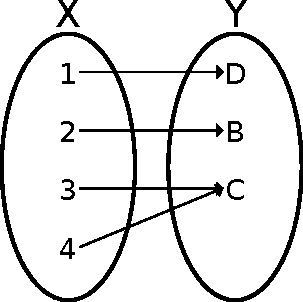
\includegraphics[width=3cm]{Surjection.pdf}}\hfill
\subfigure[injektive
Abbildung]{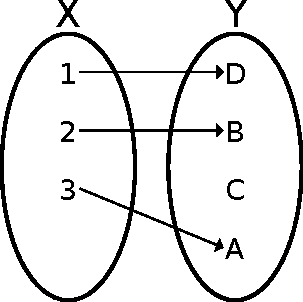
\includegraphics[width=3cm]{Injection.pdf}}\hfill
\subfigure[bijektive
Abbildungen]{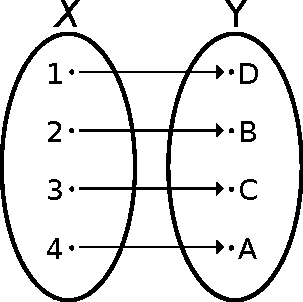
\includegraphics[width=3cm]{Bijection.pdf}}\hfill
\subfigure[identische
Abbildungen]{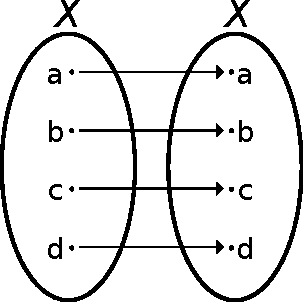
\includegraphics[width=3cm]{Identitaet.pdf}}
\end{figure}

\subsubsection{Mächtigkeit von Definitions- und Wertebereich}

Für Surjektionen gilt: $|A| \geq |B|$

Für Injektionen gilt: $|B| \geq |A|$

Weil für bijektive Abbildungen beide Aussagen gelten müssen gilt:
$$|A| \geq |B| \wedge |B| \geq |A| \Rightarrow |A| = |B| $$


Analog gilt auch:
$$ |A|<|B| \Longleftrightarrow \Surj(A,B) = \emptyset $$
$$ |A|>|B| \Longleftrightarrow \Inj(A,B) = \emptyset $$
$$ |A| \neq |B| \Longleftrightarrow \Bij(A,B) = \emptyset $$

Die ersten Aussagen schließen von einem Typ von Abbildung auf die Mächtigkeit von Definitions- und Wertebereich.
Die drei letzen Aussagen schließen von Definitions- und Wertebereich auf die (nicht) möglichen Typen von Abbildungen.

Würden die Beziehungen zwischen den Mächtigkeiten nicht gelten, würde z.B. die
Formel zur Mächtigkeit von $\Inj(A,B)$ zu Widersprüchen führen(vlg. nächstes
Kapitel).
